\chapter{Introduction}
\label{cpt:intro}
The appearance of a scene can often give us an abundance of information about the scene including time of day, location, and weather. With all of this information available, it is up to us to find ways to automatically extract it from images of the scene to allow us to better understand what is going on at a given location. In this thesis we will attempt to use the information collected by webcams to infer information about environmental signals such as wind speed \& direction and vapor pressure. 

The challenge is that images may vary more due to other causes such as time of day than those which relate to our signals of interest. Thus, we begin by exploring mechanisms for learning features that are invariant to other scene changes. Through the use of correlation techniques such as Canonical Correlation Analysis (CCA), we find that we are able to extract useful information from webcam images which allow us to predict local weather data and as a result gain better understanding of local weather patterns and variations and fill in missing weather data entries, which occur quite frequently. Furthermore, this allows us to use the abundantly existing webcams all over the country as crude weather sensors instead of depending only on the government weather stations sparsely spread out across the country. 

This thesis will go through the background information, motivation, and related work in Section \ref{cpt:intro}. It will then discuss the theory and details of the correlation techniques used in Section \ref{cpt:cca}. Section \ref{cpt:results} will begin to show the application and results of the aforementioned methods. It will also show how we further utilize our results to determine the appropriate size of the training set necessary to avoid any inherent bias in the images. We will conclude in Section \ref{cpt:conclusion} and propose future work on this problem in Section \ref{cpt:future}.

\section{Related Work}
The work presented in this paper is primarily related to two areas of research in computer vision; here we will present some of the work related to algorithms designed to operate on webcam image sequences as well as the use of CCA and other correlation techniques to extract external signals from time-varying image sequences.

\textbf{TODO}

\section{Background Information}
The Archive of Many Outdoor Scenes (AMOS) database \cite{jacobs07amos} has been collecting images from 835 webcams every 30 minutes since March 2006 and now contains over 40 million images. The AMOS dataset is unique in providing time-stamped images from many cameras around the world. No other dataset provides the broad range of geographic locations and the long temporal duration.This database is the largest known collection of natural scenes collected from static cameras and as such offers a wealth of data to test our methods against. While there are cameras located across the world, we focus on those located within the continental United States so that we can collect accurate ground truth weather data.

Our weather data is collected from the Historical Weather Data Archives (HWDA) \cite{noaa} which is maintained by the National Oceanic and Atmospheric Administration (NOAA), which is an official government organization. The archives maintain a large variety of weather data from the since January 1, 1933 through present day on just over 6,000 weather stations across the continental United States. The data collected includes, but is not limited to, wind speed \& direction, precipitation, temperature, relative humidity, vapor pressure, cloud conditions, dew point, and various aggregated data signals.

\chapter{Canonical Correlation Analysis (CCA)}
\label{cpt:cca}
The main correlation technique which we will explore is a method called Canonical Correlation Analysis (CCA) \cite{hotelling}. The goal of CCA is to find two transformation matrices $A$ and $B$ to maximize the correlation between two independent data sets $X \in \mathbf{R}^{x\times n}$ and $Y \in \mathbf{R}^{y\times n}$. In other words, CCA looks to find $A$ and $B$ such that $AX\approx BY$. CCA is a way of finding a linear relationship between two independent, multidimensional variables.

\textbf{MORE}

What makes CCA different from other correlation methods is its invariance to affine transformations of the input variables. In other words, CCA will be able to find a linear relationship between two multidimensional variables even if different coordinate systems are used for each variable \cite{bkl97}. This makes CCA a very desirable method for relating image data to environmental signals, which are clearly not measured in the same coordinate system. One very crucial component of CCA is that while the input matrices $X$ and $Y$ can have a varying number of dimensions, they must have \textit{exactly} the same number of samples in order to find an accurate correlation between the two time-varying signals.

\section{Applications}
We will now focus on the application of CCA to predicting time-varying weather signals from image sequences over the same time period. Given the localized nature of weather data, we assume that the weather station used for ground truth weather data is located near to the camera in order to maximize the accuracy of our predictions. The algorithm takes as input a set of images $I=i_1\ldots i_a$ and a set of weather observations $W=w_1\ldots w_b$. The method will assume the availability of images and weather data with corresponding timestamps. In order to ensure that this invariant holds, the first step of our algorithm is to run through both data sets and remove entries that do not have a corresponding entry in the other dataset. This step guarantees that all of our data samples match and that there are an equal number in both sets, which is required for CCA. Our input is now of the form $I=i_1\ldots i_n$ and $W=w_1\ldots w_n$.

\begin{figure}
	\centering
		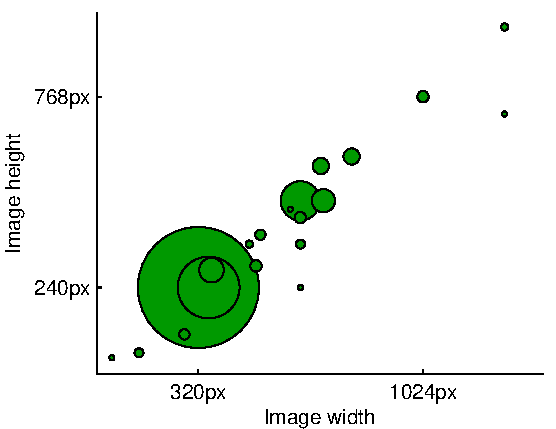
\includegraphics{figures/imagedimensions.pdf}
	\caption{The distribution of image sizes, measured in pixels. The circles are centered at the width and height of the image and their sizes are proportional to the number of webcams which output images of that size in the AMOS dataset.}
	\label{fig:imagedimensions}
\end{figure}

Once our datasets are properly aligned, we turn our attention to the images. Figure \ref{fig:imagedimensions} shows us that the most common size image from a webcam in the AMOS dataset is $320\times 240$ pixels, which means that we can express $n$ image as a $n\times 76800$ matrix. This is clearly a very costly and inefficient way to store image data, especially when we are looking to run CCA with a few hundred images. In order to reduce the storage size for each image, and as a result accelerate the runtime of our algorithms, we will run Principal Component Analysis (PCA) on the images as a way to extract the $k$ most important features from the images and then express each image as a linear combination of these features (we will use $k$=10). PCA will extract significant scene variations from the set of input images which maximize the covariance of the dataset. We will then look to use these coefficients as input to CCA. PCA will take as input a set of images $I$ and will return three matrices $U\in \mathbf{R}^{m\times k}$, $S\in \mathbf{R}^{k\times k}$, and $V\in \mathbf{R}^{k\times n}$ where $m$ is the length of a single image when expressed as a vector. $U$ contains the $k$ feature vectors, $S$ is a diagonal matrix, and $V$ contains the coefficients of each of the $k$ feature vectors for each of the $n$ images. We can thus create reconstructions of the images by multiplying $U$, $S$, and $V$ back together.

The PCA coefficients for each image stored in $V$ and our corresponding weather data $W \in \mathbf{R}^{y\times n}$ will be our input matrices for CCA. After running CCA, we will have projection matrices $A$ and $B$. We can now use these to predict weather data from new images which were not included in the input for CCA. Given a new image $i$, we begin by obtaining the $k$ PCA coefficients by projecting the image onto our existing basis vectors stored in $U$. We can now take those coefficients in a vector $\mathbf{v}$ and use them to predict the associated weather values $\mathbf{w}$ as follows:
\begin{equation}\mathbf{w}=A\mathbf{v}B^{-1}\end{equation}
This is the key equation that is used to extract the inherent weather data from an image. We will now begin to apply these algorithms to actual data sets and present some results as well as additional information we can extract with regards to minimum size of the training set and the orientation of the camera.

\chapter{Results \& Analysis}
\label{cpt:results}
We consider two weather signals for our driving examples: wind velocity and vapor pressure. These two signals present unique challenges and opportunities. The effect of wind velocity is limited to locations in the scene that are affected by wind, such as flags and vegetation. On the other hand, vapor pressure may affect the scene in a more broad and subtle manner. Choosing two examples with such unique characteristics is a great way to test whether our algorithm is able to handle any variety of weather signals or if it can only handle certain types of measurements.

\section{Wind Speed \& Direction}
Our first driving example of this method will be using wind velocity. Wind is a variable whose effects are only seen in certain local parts of the image; objects such s building and cars will be unaffected by changes in wind. In order to ensure that we could accurately predict the wind, we chose a camera which contained a flag (Figure \ref{fig:windspeedextremes}). 
\begin{figure}
	\centering
		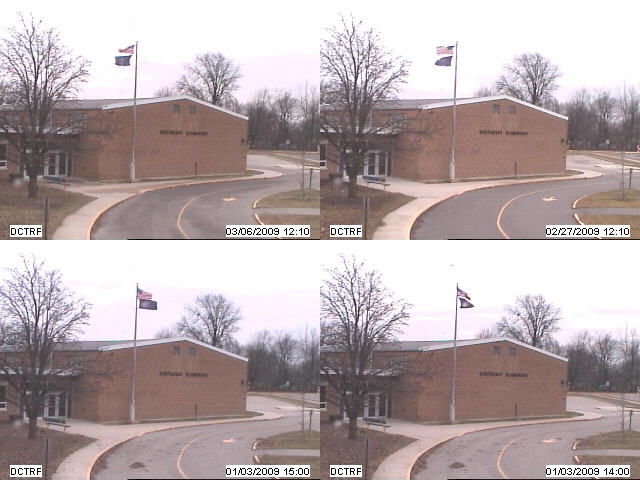
\includegraphics[width=0.70\textwidth]{figures/windspeedextremes.jpg}
	\caption{Some sample images from camera $\#$194 of the AMOS database located in Decatur, IN. The presence of a flag on top of the school building is key to our ability to predict wind speed and direction.}
	\label{fig:windspeedextremes}
\end{figure}

Our CCA projections are trained on 204 images collected between January 1 and February 11, 2009. In order to focus on variations in the scene due to weather, we only use images captured between 10 AM and 2 PM local time. By doing this we can successfully remove most of the variation caused by time of day and the resulting shadows. The wind data is made up of a wind speed and a direction in degrees, which we convert to north/south and east/west components, and was collected from the closest weather station to the camera. After running CCA, we can project matrix $A$ onto our feature vectors $U$ from the PCA analysis of the images to visualize the canonical features extracted by CCA. As we see in Figure \ref{fig:windspeedcomponents1}, CCA clearly identifies the position of the flag as the crucial indicator of wind speed. Furthermore, we can also notice slight variations in the tree positions, which also are affected by wind speed.
\begin{figure}
	\centering
		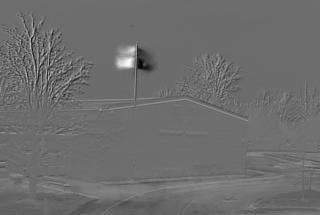
\includegraphics[width=0.55\textwidth]{figures/windspeedcomponents1.jpg}
	\caption{The projection of the first basis vector from CCA onto the original image space. It is clear to see that the position of the flag and the trees are the major variations.}
	\label{fig:windspeedcomponents1}
\end{figure}

\begin{figure}
	\centering
		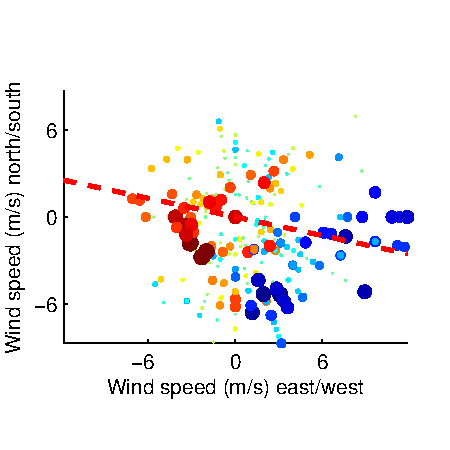
\includegraphics{figures/windspeedscatter.pdf}
	\caption{Further analysis of the wind speed predictions provides a way for us to predict the axis along which the flag is blowing. The size and color of each marker is determined by the predicted wind speed and the location of each marker is determined by the north/south and east/west components of the actual wind speed at the same time. The dashed red line is the normal to the projection axis determined by running linear regression between the predict and actual values.}
	\label{fig:windspeedscatter}
\end{figure}

\section{Vapor Pressure}

\section{Error Analysis}
A standard question that must be asked of any machine learning algorithm is: how large of a training dataset is necessary to build an strong model? A strong model is on that can predict our given weather data both accurately \textit{and} precisely. That is, our predictions from novel data have small error residuals and are not biased in one direction or the other. The combination of accuracy and precision is a strong argument that our model is truly predicting weather data and not some other signal from the image that is similar to the weather. The goal now is to find the minimum number of data samples which we need to build such a model. 

Prior work \cite{barcikowski} using Monte Carlo simulations has suggested that CCA requires the size of the training dataset to be between 40 and 60 times the number of variables being used in correlation analysis. While this may be true for general cases, we will argue here that a far smaller amount is required if the samples sufficiently cover the distribution of possible values.


\chapter{Conclusion}
\label{cpt:conclusion}

\chapter{Future Work}
\label{cpt:future}